%%%%%%%%%%%%%%%%%%%%%%%%%%%%% Define Article %%%%%%%%%%%%%%%%%%%%%%%%%%%%%%%%%%
\documentclass{report}
%%%%%%%%%%%%%%%%%%%%%%%%%%%%%%%%%%%%%%%%%%%%%%%%%%%%%%%%%%%%%%%%%%%%%%%%%%%%%%%
%%%%%%%%%%%%%%%%%%%%%%%%%%%%% Using Packages %%%%%%%%%%%%%%%%%%%%%%%%%%%%%%%%%%
\usepackage{geometry}
\usepackage{graphicx}
\usepackage{amssymb}
\usepackage{amsmath}
\usepackage{amsthm}
\usepackage{empheq}
\usepackage{mdframed}
\usepackage{booktabs}
\usepackage{lipsum}
\usepackage{graphicx}
\usepackage{color}
% \usepackage{psfrag}
\usepackage{pgfplots}
\usepackage{bm}
\usepackage{amsmath}
\usepackage[most]{tcolorbox}
\usepackage{xparse}
\usepackage{darkmode}
\usepackage[stable]{footmisc}
\usepackage{gensymb}
\usepackage{siunitx}
\usepackage[colorlinks]{hyperref}
\usepackage{fancyhdr}
\usepackage{graphicx}
\graphicspath{ {./figs/} }
\usepackage[
  backend=biber,
  sorting=none,
  % style=mla
]{biblatex}
\addbibresource{sources.bib} 


% --- Glossaries + TikZ externalization friendly setup ---
\makeatletter
\@ifundefined{pgfexternalrealjob}{%
  % Main document run: full glossaries with automake
  \usepackage[automake]{glossaries-extra}%
}{%
  % External TikZ runs: minimal glossaries that don't try to build/read files
  \usepackage[nostyles]{glossaries-extra}%
  % Pretend glossary files don't exist, so no "use \makeglossaries" error
  \def\glsifexists#1#2#3{#3}%
}
\makeatother

\usetikzlibrary{calc,decorations.pathreplacing, arrows.meta, positioning, external}


%%%%%%%%%%%%%%%%%%%%%%%%%%%%%%%%%%%%%%%%%%%%%%%%%%%%%%%%%%%%%%%%%%%%%%%%%%%%%%%

% Other Settings
\sloppy

%%%%%%%%%%%%%%%%%%%%%%%%%% Page Setting %%%%%%%%%%%%%%%%%%%%%%%%%%%%%%%%%%%%%%%
\geometry{a4paper}

%%%%%%%%%%%%%%%%%%%%%%%%%% Define some useful colors %%%%%%%%%%%%%%%%%%%%%%%%%%
\definecolor{ocre}{RGB}{243,102,25}
\definecolor{mygray}{RGB}{243,243,244}
\definecolor{deepGreen}{RGB}{26,111,0}
\definecolor{shallowGreen}{RGB}{235,255,255}
\definecolor{deepBlue}{RGB}{61,124,222}
\definecolor{shallowBlue}{RGB}{235,249,255}
%%%%%%%%%%%%%%%%%%%%%%%%%%%%%%%%%%%%%%%%%%%%%%%%%%%%%%%%%%%%%%%%%%%%%%%%%%%%%%%

%%%%%%%%%%%%%%%%%%%%%%%%%% Define an orangebox command %%%%%%%%%%%%%%%%%%%%%%%%
\newcommand\orangebox[1]{\fcolorbox{ocre}{mygray}{\hspace{1em}#1\hspace{1em}}}
%%%%%%%%%%%%%%%%%%%%%%%%%%%%%%%%%%%%%%%%%%%%%%%%%%%%%%%%%%%%%%%%%%%%%%%%%%%%%%%
%%%%%%%%%%%%%%%%%%%%%%%%%%%% English Environments %%%%%%%%%%%%%%%%%%%%%%%%%%%%%

%%%%%%%%%%%%%%%%%%%%%%%%%%%%% Theorem Macro %%%%%%%%%%%%%%%%%%%%%%%%%%%%%%%%%%%
\newtheoremstyle{mytheoremstyle}{3pt}{3pt}{\normalfont}{0cm}{\rmfamily\bfseries}{}{1em}{{\color{white}\thmname{#1}~\thmnumber{#2}}\thmnote{\,--\,#3}}
\newtheoremstyle{myproblemstyle}{3pt}{3pt}{\normalfont}{0cm}{\rmfamily\bfseries}{}{1em}{{\color{white}\thmname{#1}~\thmnumber{#2}}\thmnote{\,--\,#3}}
\theoremstyle{mytheoremstyle}

\newmdtheoremenv[linewidth=1pt,
                backgroundcolor=black!85,
                fontcolor = white!90,
                linecolor=white!100,
                leftmargin=0pt,
                innerleftmargin=20pt,
                innerrightmargin=20pt,]{theorem}{Theorem}[section]
\theoremstyle{mytheoremstyle}
\newmdtheoremenv[linewidth=1pt,backgroundcolor=shallowBlue,linecolor=deepBlue,leftmargin=0pt,innerleftmargin=20pt,innerrightmargin=20pt,]{definition}{Definition}[section]
\theoremstyle{myproblemstyle}
\newmdtheoremenv[linecolor=black,leftmargin=0pt,innerleftmargin=10pt,innerrightmargin=10pt,]{problem}{Problem}[section]
%%%%%%%%%%%%%%%%%%%%%%%%%%%%%%%%%%%%%%%%%%%%%%%%%%%%%%%%%%%%%%%%%%%%%%%%%%%%%%%


\theoremstyle{myproblemstyle}
\newmdtheoremenv[
  linecolor=black,
  leftmargin=0pt,
  innerleftmargin=10pt,
  innerrightmargin=10pt,
]{example}{Example}[section]



%%%%%%%%%%%%%%%%%%%%%%%%%%%%%%%%%%%%%%%%%%%%
%%%%%%%%%%%%%%% Equation Macro %%%%%%%%%%%%%
%%%%%%%%%%%%%%%%%%%%%%%%%%%%%%%%%%%%%%%%%%%%

% Simple mdframed style for equation boxes (no TikZ)

\enabledarkmode

\newmdenv[
  linewidth=0.8pt,
  linecolor=white,
  backgroundcolor=black!85,
  fontcolor=white!90,
  roundcorner=3pt,
  skipabove=12pt,
  skipbelow=12pt,
]{quoteBox}


\newmdenv[
  linewidth=0.5pt,
  linecolor=white,
  backgroundcolor=black!80,
  fontcolor=white!90,
  roundcorner=3pt,
  leftmargin=0pt,
  rightmargin=0pt,
  skipabove=\baselineskip,
  skipbelow=\baselineskip,
  innertopmargin=6pt,
  innerbottommargin=6pt,
  innerleftmargin=6pt,
  innerrightmargin=6pt
]{eqbox}

\ExplSyntaxOn
\seq_new:N \g_piers_eq_seq

% Store (label, title, equation-body) for later printing
\cs_new_protected:Npn \piers_add_eq:nnn #1#2#3
  {
    \seq_gput_right:Nn \g_piers_eq_seq
      { \piers_eq_entry:nnn {#1}{#2}{#3} }
  }

% How each equation is printed in the final summary
\cs_new_protected:Npn \piers_eq_entry:nnn #1#2#3
  {
    \par\noindent
    \begin{minipage}{0.72\linewidth}
      \begin{equation*}
        #3
      \end{equation*}
    \end{minipage}
    \begin{minipage}{0.9\linewidth}
      \raggedright
      \qquad\eqref{#1}\;(\textit{#2})
    \end{minipage}

    \par\bigskip
  }

% Environment: \begin{eqboxed}{label}{Title}{Description} <equation> \end{eqboxed}
\NewDocumentEnvironment{eqboxed}{ m m m +b }
  {
    % begin code: mdframed-based, no TikZ
    \begin{eqbox}
      {\bfseries #2}\par\vspace{0.4em}%
      \begin{equation}
        \label{#1}
        #4
      \end{equation}
      #3
    \end{eqbox}
    % store equation body for later
    \piers_add_eq:nnn{#1}{#2}{#4}
  }
  {
    % end code
  }

% Command to print all stored equations at the end
\NewDocumentCommand{\PrintAllEquations}{}
  {
    \section{Equations}
    \seq_use:Nn \g_piers_eq_seq { }
  }
\ExplSyntaxOff


%%%%%%%%%%%%%%%%%%%%%%%%%%%%%%%%%%%%% custom commands %%%%%%%%%%%%%%%55%%%%%%%

\def\msun{M_\odot}


%%%%%%%%%%%%%%%%%%%%%%%%%%%%%%% Plotting Settings %%%%%%%%%%%%%%%%%%%%%%%%%%%%%
\usepgfplotslibrary{colorbrewer}
\pgfplotsset{width=8cm,compat=1.9}
%%%%%%%%%%%%%%%%%%%%%%%%%%%%%%%%%%%%%%%%%%%%%%%%%%%%%%%%%%%%%%%%%%%%%%%%%%%%%%%

%%%%%%%%%%%%%%%%%%%%%%%%%%%%%%% Title & Author %%%%%%%%%%%%%%%%%%%%%%%%%%%%%%%%
\title{Notes}
\author{Pierson Lipschultz}
%%%%%%%%%%%%%%%%%%%%%%%%%%%%%%%%%%%%%%%%%%%%%%%%%%%%%%%%%%%%%%%%%%%%%%%%%%%%%%%

%%%%%%%%%%%%%%%%%%%%%%% Glossary entries %%%%%%%%%%%%%%%%%%%%%%%%%%%%%%%%%%%%%%

% Only do the real glossaries work in the main document run
\tikzifexternalizing{}{%
  \makeglossaries
}

\tikzexternalize[prefix=tikz-cache/]
%%%%%%%5%%%%%%%%%%%%%%%%%%%55



\makeglossaries 
\loadglsentries{subTex/Astro-glossary} % no .tex extension



\begin{document}
    \pagestyle{fancy}

    \fancyhf{}
    \fancyfoot[L]{\nouppercase{\leftmark}} % "1 INTRODUCTION"
    \fancyfoot[R]{\thepage}                               % page number on right

    % Remove header rule and add footer rule instead
    \renewcommand{\headrulewidth}{0pt}
    \renewcommand{\footrulewidth}{1pt}
    \renewcommand{\sectionmark}[1]{\markboth{#1}{}}

    \tableofcontents

\pagebreak

\part{Class Notes}
\chapter{Astro210}
\input{classNotes/astro210.tex}


\part{Paper Notes}
% Paper chapters are included from mainNotes via paperIncludes.tex.
% New notes register a \subfile{...} line in paperIncludes.tex (see scripts/new-paper.py).

\documentclass[../../mainNotes.tex]{subfiles}
\begin{document}

\chapter{Elusive hot stripped helium stars in the Galaxy \cite{yungelsonElusiveHotStripped2024}}
\hrule
\vspace{.5cm}

\section{Stripped Helium Star Properties}

\begin{list}{-}{}
\item non\gls{Degenerate-matter} He-cores of which retained a \(\lesssim 1 M_\odot\) hydrogen-helium envelope.  This chemical abundance is formed by numerous aspects
\begin{list}{-}{}
\item the retreat of an H-burning convective core in MS 
\item Mixing! 
\item Mass loss during RLOF 
\item Stellar wind from a post RLOF remnant
\end{list}
\item Masses of \((1-7)M_\odot\)
\item None have been identified 
\item Most are lower mass \((\gtrsim 2M_\odot)\)
\item Their formation is heavily constrained by \gls{runaway-RLOF} 
\item Likely progenitors of both hydrogen-poor and hydrogen-rich core-collapse SNe, occurring when their CO core exceeds \(\approx 1.4 M_\odot\)
\item stars with mass \(\lesssim 2M_\odot\) with hydrogen-depleted envelopes are sdO/B-type subdwarf and stripped stars with mass \(\gtrsim 7M_\odot\) are Wolf-Rayet stars. This gap is believed to be filled with HeS stars 
\item 
\end{list}

\section{Case B RLO}\label{Yungelson-case-b-rlo}
``At solar metallicity \(Z = Z_\odot\) this results in the formation of a system with a He white dwarf component, if the \gls{ac:ZAMS} donor mass is \(\lesssim 2.5 M_\odot\) or a hot \((\log(T_{eff} \lesssim 4.4))\) stripped helium star (HeS) component, if the donors ZAMS mass is higher and the mass-loss by its stellar wind does not prevent RLOF'' 

\end{document}


\pagebreak
\chapter{An upper limit on the frequency of short-period black hole companions to Sun-like stars \cite{green_upper_2025}}
\hrule
\vspace{.5cm}
\section{Abstract}
\hrule
\vspace{.5cm}
\begin{list}{-}{}
\item Seeking to narrow the uncertainty regarding the survival rate in the formation of stellar-mass BHs. 
\item This uncertainty is most extreme in LMXB systems
\item Defines `close' systems as  \(P_{orb} \lesssim 3\text{d}\) 
\item Searching through for AFGK-type stars in \gls{TESS}\footnote{I wonder why TESS was picked}. These are the \textit{\textbf{non-accreting}} companion and progenitors of LMXBs
\item Detecting the BHs via the deformation of the main star via the light curves 
\item Found a selection of 457 candidates from a sample of \(4.7 \times 10^6\)
\item However, after spectra follow-up on 200 of the sample, \textit{none showed spectra consistent with a BH companion}\footnote{Very curious what ``spectra consistent with a BH companion'' means, especially as these are non accreting. Is this using a radial velocity method?\dots}
\item On the basis on non-detection they conclude that fewer than one in \(10^5\) \textit{sun-type} stars host a \textit{close} BH companion
\item This upper limit is in tension with that some models predict (\(\sim10^{4-5}\)), but congruent with other models that predict on in \(10^{7-8}\)
\end{list}

\pagebreak
\section{Introduction}
\hrule
\vspace{.5cm}
\begin{list}{-}{}
\item Isolated stars with mass greater than \(\gtrsim 15-25 M_\odot\) are believed to end their lives as BHs, suggesting that there are \(\sim 10^8\) stellar mass BHs in our galaxy. The majority of which are believed to evolve with a stellar companion, half of which will interact with said companion at some point during their lifespan.
\item A very small number (7) \gls{BH_LS} systems have been detected
\item Because of the scarcity of these systems, it's useful to try and set an upper limit on their distribution
\end{list}


\input{paperNotes/sunLikeStarKareemElBardy/sunLikeStar.tex}



\part{General Notes}
\chapter{Misc}
\hrule
\vspace{.5cm}
\section{WD SNe}\label{WD-SNe}
\hrule
\vspace{.5cm}
\begin{list}{-}{}
\item This, simply-ish put, is caused by because a WD cannot reach hydrostatic equilibrium. A pressure increase does \textbf{not} lead to increase and radius, and thus cooling, instead, it just increases heat, and thus fusion, quickly getting out of hand. Can b trigged if the \gls{chandrasekhar-limit} is crossed, as well as if a layer of H/He on top entities, called a \gls{edge-limit-detonation} or ``sub-Chandrasekhar'' explosions.
\item In \gls{ac:DD} systems the WDs must have a small separation, causing \gls{ac:GWR} to shrink the separation until merger \(\rightarrow\) SNe
\end{list}

\section{Pauli Exclusion Principle}\label{pauli-exclusion-principle}
\hrule
\vspace{.5cm}
The property of matter that two identical particles with half integer spins (fermions) cannot occupy the same quantum state. \\
\begin{quoteBox}
\url{https://en.wikipedia.org/wiki/Pauli_exclusion_principle} \\ 
``In a poly-electron atom it is impossible for any two electrons to have the same two values of all four of their quantum numbers, which are: n, the principal quantum number; \(\ell\), the azimuthal quantum number; \(m\ell\), the magnetic quantum number; and ms, the spin quantum number. For example, if two electrons reside in the same orbital, then their values of n, \(\ell\), and \(m\ell\) are equal. In that case, the two values of \(ms\)(spin) pair must be different. Since the only two possible values for the spin projection \(ms\)are +1/2 and -1/2, it follows that one electron must have \(ms\)= +1/2 and one \(ms\)= -1/2.''
\end{quoteBox}
This means that in systems of very dense matter, the system \textit{\textbf{{cannot reach homogeneity}}}, and thus will actually have an inherent pressure. This pressure can prevent collapse due to gravity in various high dense objects (compact objects in astronomy).

\pagebreak
\section{Relativistic Beaming}\label{sec:RelBeaming}
\hrule
\vspace{.5cm}

The process of an object becoming brighter when it is moving \textit{towards} the Earth. This is \textit{in conjunction} with Doppler shift. This brightness increase can be attributed to the fact that, for a star moving \textit{towards} the earth, from the perspective of the earth, a `clock' placed near the star would run \textit{faster} than one on earth. If photons are emitted at a set rate on this `clock' it would be faster, when scaling the star `clock' to the earth one, it would be faster, meaning that the interval between received photons would be faster, and thus the object would appear brighter.  

\section{Ellipsoidal Modulation}
\label{sec:ellipsoidalModulation}
\hrule
\vspace{.5cm}
See \url{https://agn.caltech.edu/~srk/Ay215/Presentations/ellipsoidal_mod.pdf}!!!



\pagebreak
\section{Gravitational Waves}
\label{sec:Gravitational-Waves}
\hrule
\vspace{.5cm}

\begin{list}{-}{}
\item Ripples in spacetime created by relative acceleration of massive objects. 
\end{list}

\subsection{Observational Properties in BBHs}
\hrule
\vspace{.5cm}
\begin{list}{-}{}
\item Using a GW obs one can obtain the spins and masses of merging BHs
\item Spins have a magnitude (speed of rotation) and direction (axis of rotation)
\end{list}


\part{\textit{Physics of Binary Star Evolution} Notes \cite{TaurisvandenHeuvel+2023}}
\setcounter{chapter}{0}


\chapter{Intro}
\hrule
\vspace{.5cm}

\noindent \textbf{\large Importance of binaries}
\begin{list}{-}{}
\item Plays a key role in the evolution of massive stars
\item first presumed to exist because of \gls{algol-type} stars. These stars were explained with mass transfer
\item Mergers are a key source of strongest GW rad, GrBs, and have r-process elements. (i.e. in \gls{kilonova}) 
\item Likely cause of SNe Ia, Ib, Ic (SN with a lack of hydrogen in their spectra) 
\item cause of low-intermediate mass stars with odd chemical compositions, ex. barium stars. 
\end{list}

\pagebreak
\chapter{Visual binaries and the universal validity of the laws of physics}
\hrule
\vspace{.5cm}


\section{Visual binaries}
\begin{list}{-}{}

\item Visual binary \(\rightarrow\) two in proximity through a telescope

\item Physical \(\rightarrow\) gravitonalty bound orbits

\item Optical \(\rightarrow\) happen to be close together in the sky

\end{list}

\begin{list}{-}{}
\item Visual binaries have longer orbits
\item the proof of physical binaries (and not just coincidence) was proved in 1767 by John Michell
\item Shows that Newton's law of gravity applied outside just our solar system
\end{list}
\section{Astrometric Binaries}
\noindent \textbf{\large Wide binaries} 
\begin{list}{-}{}
\item Binaries where one of the stars is too faint to directly observe
\item Can still be detected by the following \gls{proper-motion} of the visible component
\item Center of mass moves along, star orbits this center, showing a periodic wiggle in its apparent motion (I wonder how this can be muddled with and/or separated from parallax. I'm guessing they are in different planes?? (next graphic helped(it wiggles slightly due to yearly parallax, however, the proper motion is much greater and over a much longer duration, so it sort of just becomes ``noise'' relative)))
\end{list}
\section{Spectroscopic Binaries}
\noindent \textbf{\large Spectroscopic Binaries}
\begin{list}{-}{}
\item A binary which is determined to be a binary due to its spectra
\item double-lined binary (SB2) \(\rightarrow\) when both sets of spectral lines can be observed redshifting and blueshifting
\item single-lined (SB1) \(\rightarrow\) when only set of spectral lines can be observed redshifting/blueshifting
\item this is due to Doppler shifting when one of the binaries is relativistically coming towards us and the other away
\item Doppler shift (\(\Delta\lambda\)) can be related to the radial velocity (the component of the velocity on our line of sight)
\item \[\frac{\Delta\lambda}{\lambda} = \frac{v_{rad}}{c}\]
\end{list}
\section{Eclipsing Binaries}
Binaries where one star passes in front of the other at some point during its period
\begin{list}{-}{}
\item A partial eclipse will happen if  
\item \[\sin(\phi) < \sin(\phi_0) = \frac{R_1+R_2}{a}\]
\item where inclination \(i\) is defined as the angle between the orbital plane and the plane of the sky \(\rightarrow\) \(\phi = 90 \degree - i\) and \(a\) is the orbital radius  
\item and a total eclipse will occur if 
\item \[\sin(\phi) < \sin(\phi_1) = \frac{R_1-R_2}{a}\]
\item We assume that the angles between line of sight and orbital planes are random, the probability of having an angle between 0 and \(\phi_0\) is the fraction of the surface area of the half sphere between the pole and the circle at an angle \(\phi_0\) from the pole, which is equal to \(2\pi(1-\cos(\phi_0))\). While the area of the half sphere is \(2\pi\)\footnote{Try this myself and verify that this makes sense}. Thus, the probability of having an eclipse is 
\item \[\mathcal{F}_{eclipse} = (1-\cos\phi_0)\]
\item Assuming \(\phi_0\) small
\item \[\sin\phi \simeq \phi_0 \simeq \frac{(R_1 +R)_2}{a}\]
\item due to series expansion\footnote{for sure do this at some point}
\item \[\cos\phi_0 \simeq 1 - \frac{(R_1 + R_2)^2}{2a^2}\]
\item Thus
\item \[\mathcal{F}_{eclipse} =\frac{(R_1 + R_2)^2}{2a^2} \]
\item Because \(R_1 +R_2 < a\), eclipses are most likely for either dwarf stars with a  very close orbital radius, or wide binaries where at least one star is a giant 
\end{list}

\section{}
\begin{list}{-}{}
\item It is possible for a spinning WDs to show variation (but not pulses) in star brightness
\item This is because of the magnetic fields on WDs causing bright spots
\item Pulsation can be determined by the density 
\end{list}
\noindent \textbf{\large Novae/CVs}
\begin{list}{-}{}
\item Caused my mass transfer onto a WD
\item WD shell goes SN, causing Novae
\item Standard candle
\item Has a variation called dwarf Novae 
\item caused by instability in the accretion disk
\item much weaker
\end{list}

\section{}
\begin{list}{-}{}
\item Brightest sources of x-rays were found to be CV accreting systems
\end{list}

\section{}
\begin{list}{-}{}
\item The first NS star XrB
\item Regular periodicity of with increase of x-ray emission
\item Caused by the NS being obscured by the larger star
\end{list}

\section{First BH XrB}
\begin{list}{-}{}
\item Discovered x-ray source with nearby supergiant
\item Falls into two classes
\item HMXBs and LMXBs
\item determined by the mass of the acceptor with respect to the donor
\item x-ray emission called by infilling matter
\item \(\frac{GMm}{R} = .01mc^2\)\footnote{Shockingly simple eq}
\item much much much more efficient than any fusion reactor on earth
\item values as high as \(.42mc^2\)
\item Common in Globular clusters
\end{list}

\section{Double NSs \& BHs}
\begin{list}{-}{}
\item Proved by GW detection
\item Detections are dominated by DBHs 
\item DNSs formed through lower mass binaries
\end{list}

\section{MSPs}
\begin{list}{-}{}
\item Generally remnants of LMXBs
\item Systems with \gls{MSP}s generally have WD partners
\item Mass-transfer through evolution, or through orbital momentum loss through or GWR
\item The NS is greatly accelerated through accretion
\item Old NSs which evolved through this process are called \textit{\gls{Recylced-Pulsar}s}
\end{list}

\section{Results of evolution in binaries}
\begin{list}{-}{}
\item SNe caused by the death of stars more massive than \(\sim8M_\odot\)
\item SNe types
\begin{list}{-}{}
\item \gls{TI-SNe}
\item \gls{TIb-SNe}
\item \gls{TIc-SNe}
\item \gls{TII-SNe} 
\end{list}
\item due to the fact that \gls{TIb-SNe} and \gls{TIc-SNe} are stripped cores, it is incredibly likely that they result from binary systems
\item We may also observe both \gls{TIb-SNe} and \gls{TIc-SNe} in \gls{WR-star}, however, we have \textbf{not} yet
\item WD SNe (section \ref{WD-SNe}) \textit{require} some sort of mass transfer process
\item The companion donor can be either a standard star (\gls{SD}), or another WD (\gls{DD})
\end{list}

\section{Weird stars}
\begin{list}{-}{}
\item Blue stragglers
\item Barium 
\end{list}


\pagebreak
\chapter{Orbits and masses of spectroscopic binaries}
\hrule
\vspace{.5cm}

\setcounter{subsection}{3}
\section{}
This is generally all math that I either know from astro classes, or is so specific id need to revisit it to use anyway\\

\[\frac{L}{L_\odot} = \frac{M}{M_\odot}^{3.5}, M > 1.3M_\odot\]

\section{Very massive stars}
\begin{list}{-}{}
\item Most massive has \(L \sim 10^ L_\odot\)
\item Because of the high (\(\sim50000k\)) temps, they have strong stellar wind, and thus very similar spectra to \gls{WR-star}, which they are distinguished from by the presence of hydrogen 
\item Denoted as \gls{WNh}
\end{list}

\section{Stuff that screws up rad vel curves}
\begin{list}{-}{}
\item Rad Vel curve must be off due to a difference in eccentricity values derived from the rad curve and the light curve
\item Rotation effect
\begin{list}{-}{}
\item when the stars are eclipsing the rotational Doppler shift can be added (if the half spinning away from us is obscured) or subtracted to the shift, leading to different rad velocity measurements. This is called the Rossiter-McLaughlin effect. \footnote{This is actually a super neat and intuitive process which i feel like the book just sorta skips and doesnt explain, maybe wanna write out/make some graphics bout this sometime}
\end{list}
\item presence of gas streams
\begin{list}{-}{}
\item wow they could have said literally anything about what a gas stream is in this case
\item im guessing it means some sort of flow of mass coming off of the binaries, maybe in accretion, maybe in jets???
\end{list}
\item reflection effect
\item heating effect
\begin{list}{-}{}
\item Both the reflection and heating effect are caused by that the stars will cast light on each other, both heating and causing reflection
\end{list}
\item deformation effect
\begin{list}{-}{}
\item the above effects cause the curve to be shifted from the c.m., leading to wonky radial vel curves
\end{list}
\item  this is actually pretty important when it comes to HMXBs and properly measuring NS and BH masses
\end{list}


\section{Interacting binaries}
\begin{list}{-}{}
\item \(> 70\%\) of massive o-type stars are members of binaries so close that they'll exchange mass or merge before either star explode as a SN

\end{list}
the rest of this section follows the ``way too niche of math to write down'' thing

\pagebreak
\chapter{Roche equipotential}
\textit{\small I have a ridiculous amount of notes and a whole essay written about this, so notes here will be pretty light}
\vspace{.1cm}
\hrule
\vspace{.5cm}

\begin{list}{-}{}
\item This is some black magic mathmathmatic reasoning 
\item Co-rotating binaries with have a tidal bulge that can be `easily' calculated
\item also love the seemingly kinda personal rant about how the RL diagram is actually wrong, then provides a diagram which is way less intuitive  
\end{list}

\section{Mass transfer Galore}
\begin{list}{-}{}
\item Mass transfer through \(L_1\) does not majority effect angular momentum, however, transfer through \(L_2\) does, causing a shrinkage in separation, and typically mergers
\item Different ways of modeling the transfer, depending on how you treat angular momentum with respect to the transfer
\item Orbit widens if the donor is less massive then accreter, and shrinks if the donor is more
\end{list}

\section{Types of RLO}
\begin{list}{-}{}
\item \gls{consv-RLO}
\item \gls{ML-CircumDisk}
\end{list}

\section{General Notes}
\begin{list}{-}{}
\item Mass transfer onto NS and BH are limited by the \gls{eddington-limit}
\item However, mass transferred off of the donor is at the rate of the evolution of its envelope. (\gls{thermal-timescale})
\item mass transfer off of the donor is much greater (2 to 4 orders of magnitude) then the maximum accretion rate thus, the bulk of the mass will be ``blown away''
\item if more than half of the total mass of the binary system is lost in a SN, the system will become unbounded 
\item What on earth is a applegate mechanism
\item and what is gravitational quadrupole coupling
\item ^^ im pretty sure its just when the oblateness of the star various from some convection stuff, which causes the period to variation causing period variations 
\end{list}

\section{Stability Criteria}
\begin{list}{-}{}
\item Depends on the response of the star losing mass as well as the RL
\item more likely to detect it if the mass transfer is stable 
\item orbit always expands for \(q < 1 \) and always shrinks when \(q = 1.28\)
\item Depends on whether the donor contracts or swells upon starting to transfer mass
\item Donors with radiative envelopes (\gls{Case-A-RLO}) or slightly convective envelopes (early \gls{Case-B-RLO}) will typically either shrink or stay the same radius
\item 
\end{list}

\section{Tidal Evo}
\begin{list}{-}{}
\item Grav interaction will cause Tidal Bulges to form
\item If rotation of the stars is not synced with orbital motion, the movement of the bulges will cause friction, thus dissipating the KE of the star.
\item If the orbit is eccentric, the effect is greater in magnitude
\item This leads to the orbit becoming perfectly circular 
\item Happens faster in systems with closer separations
\item Tempature can heavily effect orbtial eccentrictiy based on convection rates
\end{list}

\section{CE}
\begin{list}{-}{}
\item Trigged by unstable runaway mass transfer
\item companion star is engulfed in the envelope of the donor
\item the companion moving through this envelope causing friction, thus reducing angular moment, thus shrinking orbit
\item In some cases the envelope is ejected, and if it isnt, it leads to merger
\item Likely progenitor of some planetary nebulae 
\item Very hard to predict due to unstable nature
\item Onset is caused by runaway RLO, Darwin instability, or the expansion of the accreting star
\end{list}

\subsection{Stages of CE}
\begin{list}{-}{}
\item loss of co-rotation
\item plunge-in
\item Slow spiral-in
\item Envelope Ejection
\end{list}

\subsection{CE ejection}
\begin{list}{-}{}
\item Whether not the envelope will be ejected is dependent on how good the system is at converting the GPE into KE, this added KE can then eject the envelope 
\item This can be described as the efficiency \(\alpha_{CE}\) of converting orbital energy \(\Delta E_{orb}\)
\item \[E_{bind} = \alpha_{CE}\Delta E_{orb}\] 
\item Ability to eject a CE depends heavily on the evolutionary status of the donor at the onset of CE
\item Separation post CE ejection is about 100-1000x smaller than at Onset
\item \[E_{bind} \equiv -\frac{GM_{donor} M_{env}}{\lambda R_{donor}}\]
\item \(\lambda\) various heavily on stealer mass and evolutionary status
\item For low max systems the envelopes of the donors are typically ejected, as \(|E_{bind}|\) is typically quite small
\item Many HMXBs with NSs will not survive CE and hence DNS mergers are rare, although these do theoretically form Thorne-Zytkov objects
\item 
\end{list}


\pagebreak
\setcounter{section}{7}
\chapter{Evolution of single stars}
\hrule
\vspace{.5cm}

\section{Why stars do stuff\footnote{trying to focus on some of the math here, cause while i conceptually understand it, the math is really neat}}
\begin{list}{-}{}
\item A globe of monatomic gas without energy sources and in HSEq follows
\item \[2E_{th} + E_{pot} = 0\]
\item \(E_{th}\) is given by 
\item \[E_{th} = \frac{3}{2}Nk\bar{T} = \frac{3}{2}M(\mathcal{R}/\mu)\bar{T}\]
\item Where \(N\) is the partcile number in the star, \(k\) is the boltzman constant, \(M\) is the mass of the globe \(\mathcal{R} = ak/m_h\), the ideal gas constant, \(\mu\) is the mean particle mass, in units of \(m_h\) of the hydrogen atom 
\item \(E_{pot}\) is given by 
\item \[E_{pot} = -\alpha GM^2/R\] 
\item Where \(R\) is stellar rad, \(G\) is grav const, and \(\alpha\) is a constant of proportionality of order unity, which depends on the density distribution of the star.
\item From substitution, we find that
\item \[\bar{T} = \alpha(\frac{GM}{R}) (\frac{\mu}{3\mathcal{R}})\]
\item This is import because it shows that internal temp is only depended on the stellar radius, increasing when the star shrinks
\item Energy loss is given by 
\item \[E_{tot = E_{th} + E_{pot}} = \frac{1}{2}E_{pot} = -\alpha \frac{GM^2}{2R}\] 
\item This shows that as \(E_{tot}\) decreases the radius of the star must decrease
\item However, as shown by \(\bar{T}\),as the star contracts the internal temp increases
\item This means as the star (or cloud of gas) radius heat away, it actually gets hotter, leading to more radiation, and thus more shrinking
\item This applies to the star from the moment it is a gas to the end of its life as BH, NS, WD, etc
\item These equations work well for \gls{antibiotic-index} of  \(\gamma = C_p/C_V = 5/3\), which is great for globes of ionized hydrogen and helium. However, generalized forms can be found with eqs 8.6-8.8
\item if \(\gamma \leq 4/3\), the star \textbf{cannot} reach HSEq, and thus must collapse or explode
\item Stars of very high mass have very high luminosities, which mean their interior pressure is dominated by \gls{photon-gas}, which has \(\gamma = 4/3\). This sets an upper limit for the mass of a star, also called the \gls{eddington-lum-limit}
\end{list}

\section{Stellar Timescales}
There are three timescales for single star evo that are relevant for binary stellar evo

\subsection{Dynamical Pulsation timescale}


\begin{theorem}[Dynamical-Pulsation-timescale]

  \[\tau_{dyn} = \frac{R}{c_s} \simeq 50 \text{min}\left(\frac{\bar{\rho_{\odot}}}{\bar{\rho}}\right)^{1/2}\]
  Where \(\bar{\rho}\) is the mean mass density.

  This is the timescale of how long it takes for a start to restore a perturbation of its HSEq. This can be defined as the time it takes for a sound way with velocity \(c_s\) to cross the stellar radius
\end{theorem}

\subsection{Thermal/Kelvin-Helmholtz timescale}
Timescale of how long it takes for the star to react to fusion rate not being equal to the radiative energy loss. This is import with pre-main sequence contraction and after the stars fuel has been used

\subsection{Nuclear timescale}
Time it takes for a star to use all of its available fuel

\section{High mass evolution\(M \geq 12M_\odot\)}
\begin{list}{-}{}
\item Leave behind a collapsing iron core, which creates a NS or BH 
\item 
\end{list}

\section{Low mass stellar evolution \(M\leq 8M_\odot\)}
\begin{list}{-}{}
\item The degenerate mass in the core of the star heavily effects fusion 
\item For electron degenerate gas, the pressure only depends on the density (and not on the temperature)
\item This means that this degenerate gas ignites, it has no way of stabilizing itself, leading to a `flash', where it all ignites rapidly. 
\item This will only stop when the temp reaches a point where the ideal gas is able to also do fusion, at which point the star can actually expand and cool
\item ``In stars with \(M < 2.3 M_\odot\), the core becomes degenerate during hydrogen shell burning, and when \(M_{he} \approx .47M_\odot\), the helium ignites with a flash, the temp rises to \(\approx10^9\)K, and the degeneracy is removed''
\item This is not violent to actually disrupt the star
\item In stars with mass \(2.3m_\odot < M \lesssim 8M_\odot\) they instead ignite carbon in a flash. This is strong enough to disrupt the star (albeit rarely)
\item However, it is more likely for the star to eject its helium envelope due to helium-shell burning as well as the instability of the \gls{RSG} stage, leaving behind a CO WD.
\item Because of this CO ignition is rare. 
\end{list}

\subsection{Mass limit at \(\sim 1.2M_\odot\)}
\begin{list}{-}{}
\item When hydrogen is exhausted in the star, the star contracts. This causes it to drift sharply left on the HR diagram, until the hydrogen-shell begins fusion causing it to have drift slowly upward and to the right on an HR diagram
\item 
\end{list}

\subsection{Mass limit at \(\sim 1.5 M_\odot\)}
\begin{list}{-}{}
\item Masses less than \(\sim 1.5 M_\odot\) have convective outer envelope and ones higher are radiative. 
\item This convective envelope creates a magnetic field, this magnetic field can cause \gls{magnetic-breaking}, leading to stars of this mass range having slower spins
\end{list}

\section{Stars in the range of \(8-12 M_\odot\)}
\begin{list}{-}{} \label{test}
\item Not very well is known about evolution in this range
\item Generally, the carbon in the ore will ignite and leave a degenerate \gls{ONeMg} core
\item This happens after they eject their hydrogen envelope, but in binaries this envelope is lost through mass transfer
\item This means that the ONeMg core will grow to the \gls{chandrasekhar-limit}, at which point it will then collapse, creating NS and SN explosion
\item Might also result in \gls{TI-SNe}
\end{list}


\section{Effects of wind mass loss, metallicity, and rotation}
\begin{list}{-}{}
\item If a star has very fast spin, the helium in the core can get mixed into the whole star, preventing the star from becoming a giant, instead leading it towards becoming a \gls{WR-star}\footnote{This is cool as shit. Blender star my beloved}. This can happen with stars with of low of mass as \(15M_\odot\), as compared to the typical progenitor mass of \(\sim25M_\odot\)
\item Non-rotating stars can become much more massive
% \item \gls{RSG}s are much more common which stars of higher (sun-like) metallicities
\end{list}

\section{Final Evo of stars in the range of \(1- 8 M_\odot\)}
\begin{list}{-}{}
\item Unstable pulsing
\item Very strong stellar winds
\item If they're low enough mass, (\(<8M\odot\)), they can become WDs before carbon ignition
\end{list}


\section{Final Evolution and core collapse of stars more massive than \(8M\odot\)}


\subsection{Between 8 and \(\sim 10 -12\)}
\begin{list}{-}{}
\item When the core approaches the \gls{chandrasekhar-limit} thus begins the onset of core collapse 
\item 
\end{list}



\pagebreak
\setcounter{section}{10}
\chapter{Formation and Evolution of LMXBs}
\hrule
\vspace{.5cm}

\section{Rare formation process}
\begin{list}{-}{}
\item Due to the \textit{lower} mass of the donor star when compared to the accretor, mass transfer in LMXBs can be long stable on large timescales, such as \dots
\begin{list}{-}{}
\item nuclear (fuel of the star)
\item orbital shrinking due to loss of angular momentum
\end{list}
\item When comapring the theoretical lifespan of them, to the quanity obsreved, we find that they have formation rate of \( 10^{-7} \text{yr}^{-1}\)
\item one out of \(\sim 10^{5}\) finishes in a LMXB system, whereas HMXBS it is \textit{one out of ten} 
\end{list}

\section{Possible formation channels}
\begin{list}{-}{}
\item \gls{ac:AIC} of a massive WD reaching \gls{chandrasekhar-limit} \ref{sec:LMXBAICFormation}
\item Formation Via Common Envelope Evolution \ref{sec:LMXBFormViaCE}
\end{list}
\pagebreak
\subsection{Formation Via Common Envelope Evolution\label{sec:LMXBFormViaCE}}
\hrule
\vspace{.5cm}
Deduced by looking at the Her x-1 system 
\begin{list}{-}{}
\item far distance (3kpc) from the galactic plane, but a family young star
\item must have experienced something to launch hit out of the plane at 120kms\(^{-1}\)
\item This was from an SN, most likely some sort of \gls{natal-kick}
\item The velocity of this NS is much greater than a possible value formed via \gls{ac:AIC} on a WD
\end{list}
\textbf{Evolutionary Steps}
In this config the initial system consists of a relatively massive star (\(\sim 12 \text{to} 15 M_\odot\)) together with a \(2M_\odot\) star in a wide orbit (\(P_{orb} > 1yr\)) 

\subsection{\gls{ac:AIC} of a massive WD reaching \gls{chandrasekhar-limit} \label{sec:LMXBAICFormation}}

\subsection{Origin from a HMXB with a much lower mass companion (triple star system)}







\part{AstroBites Notes}
\setcounter{chapter}{0}
\pagebreak
\chapter{What happens when you poke a black hole? \cite{Mittal2026} \label{chap:PokeABH}}
\hrule
\vspace{.5cm}

\section{Abstract and intro}
\hrule
\vspace{.5cm}
What happens when you perturb the perfect shape of a blackhole (or any other object of symmetrically and spherically distorting spacetime)?

In 1950 John Wheeler and Tullio Regge were studying spherically symmetric spacetimes outside spherical masses. Note that this was being done \textit{before} BHs were known.  

\section{How do you poke a BH?}
\hrule
\vspace{.5cm}

To `poke` a BH One can disturb the shape of its spacetime. Regge and Wheeler did this by utilizing spherical harmonics. They used two types of perturbations, \gls{odd_modes} and \gls{even_modes}. Even those these don't necessarily completely represent real physical distortions in spacetime, this simplified version became the Regge-Wheeler gauge, which serves as a modern benchmark for how these calculations are done.

\section{The Regge-Wheeler Equation}
\hrule
\vspace{.5cm}

\begin{eqboxed}{eq:ReggeWheeler}{Regge-Wheeler Equation}
{Q measures the size of a perturbation, \(r^*\) is the Turtle Coordinate \ref{eq:turtleCoordinate}, \(\omega\) is the frequency of the perturbation, and \(V_{RW}\) is an effective potential for the BHs sensitivity to perturbations. \textit{Note that this is for \gls{odd_modes}!!}}
\frac{d^2}{dr^{*2}} + \left[\omega^2 V_{RW} (r)\right]Q = 0
\end{eqboxed}

\begin{eqboxed}{eq:turtleCoordinate}{Turtle Coordinate}
{Because the Schwarzschild time coordinate approaches infinity as something (a light ray, observer, object, etc.) approaches the event horizon, it is useful to have a coordinate which approaches negative infinity in order to still allow for calculations}
r^* = r + 2GM \ln\left|\frac{r}{2GM}-1\right|
\end{eqboxed}

This equation (\ref{eq:ReggeWheeler}) looks very similar to the Schrödinger equation, allowing predictions of its behavior to be easily made. Because of this, it is easily predicted that the system will oscillate and then return to a low energy state. 

\begin{figure}[h]
    \centering
    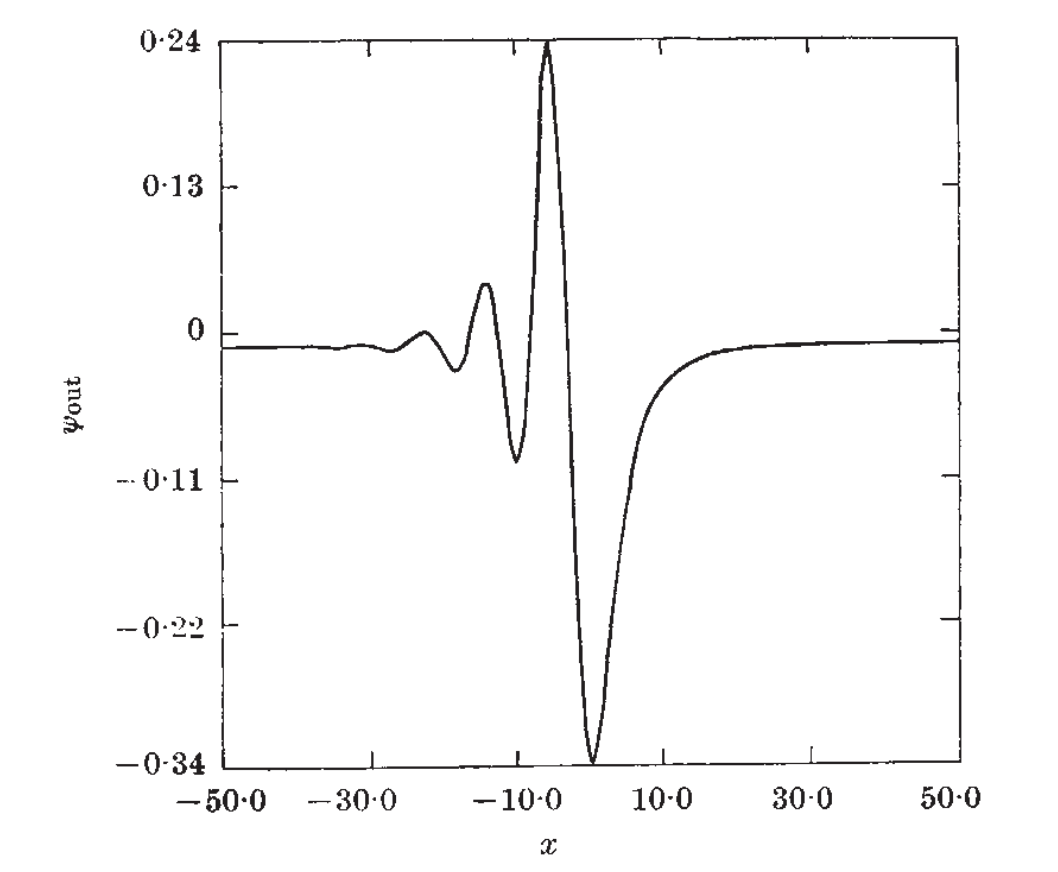
\includegraphics[width=.75\textwidth]{bhPertubation.png}
\end{figure}

The `ring-down' phase detected with LIGO after a BH merger is described using this same method.



% \pagebreak
\section{A Wandering Supermassive Black Hole Eating a Star \cite{Saad2026}}} \label{AT2024tvd}
\hrule
\vspace{.5cm}

\begin{list}{-}{}
\item Coveres a paper investigating a \gls{TDE}s dicovered \textit{away} from the center of a galaxy, denoted as AT2024tvd.
\item BH mass \texttt{determines accretion disk behavior}, with more massive BHs having larger, cooler disks
\item This can be measured with the disks' brightness  
\item This was observed with \gls{obs:Pan-STARRS}, \gls{obs:Swift Observatory}, \gls{obs:Pan-STARRS}, and \gls{obs:XMM-Newton}
\item TDEs start with an intial burst in visible and UV which is not very well understood, but after a period of time (few hundred days) the visible and UV light start to come from the accretion disk
\item Used a model called kerrSED, which measures spectral energy distribution (SED), this accounts for disk temp, physical size, spin, viewing angle, and \gls{Comptonization}
\item From this fitting they found that the BH had a mass of \(\sim M_\odot\), classifying it as a \gls{SMBH}  
\item This puts it in a unique spot, as previously detected \gls{TDE}s were located in Ultra-Compact Dwarf Galaxies, small dense collections of stars which orbit larger host galaxies.
\item AT2024tvd has nearly no surrounding stars, suggesting that it is `wandering', having being ejected form a galaxy merger and now slowly drifting towards the galactic center, sheding stars as it goes.   
\end{list}
\pagebreak
\chapter{Many Mergers Might Fill the Mass Gap \cite{Amen2026} \label{chap:ManyMergersMightFilltheMassGap}}
\hrule
\vspace{.5cm}

\begin{list}{-}{}
\item Stars of mass between 130-250 \(M_\odot\) are thought to end their lives in \gls{ac:PISN}
\item Many BHs in the mass range of 45-120 are still observed
\item The paper proposes that the BHs in this mass range are actually formed via BBH mergers, including \gls{hierarchical-merger}s. 
\item Looking to establish this theory via \gls{ac:GW} observation of hierarchical mergers.
\item 1G + 1G mergers have the same spin axis's and similar masses, as they evolved together. Whereas hierarchical mergers have differing properties
\item They created a model for both non-hierarchical and hierarchical mergers, and then combined said models with a ``mixture fraction'' to create a ``mixture model''\footnote{look into this more and add a full section or something about it :)} Fitting to this model allows for the population to filter itself into its respective subpopulations without enforcing the existence of said subpop. 
\end{list}
\pagebreak

\section{Results}
\hrule
\vspace{.5cm}
\begin{figure}[h!]
    \centering
    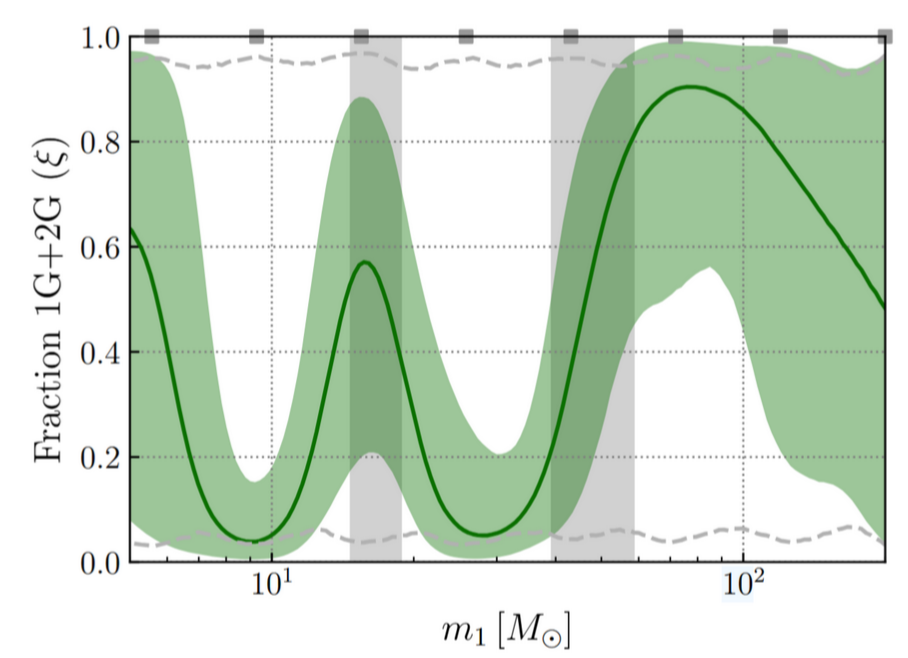
\includegraphics[width=.75\textwidth]{ManyMerger.png}
\end{figure}

We see that \dots
\begin{list}{-}{}
\item hierarchical mergers start at \(\sim 46 M_\odot\), supporting that this may fill the mass gap
\item separate collection of hierarchical mergers around 16 solar masses 
\item lack of hierarchical mergers between 20-40 solar masses
\end{list}



\printbibliography[
heading=bibintoc,
title={\centering Sources}
]

\printglossaries
\end{document}
